\documentclass[12pt]{article}
\usepackage{../common/cpp-lectures}

\title{Завдання 3. Клас Image}

\begin{document}
\maketitle
Метою цього завдання є написання класу \m{Image}, який задає API для роботи з зображенням.

\m{Image} мусить мати наступні атрибути:
\begin{itemize}
  \item зберігати розміри зображення (кількість рядків та стовпців),
  \item мати публічні методи для визначення розміру зображення по кожному виміру,
  \item метод \m{at(i, j)} для доступу (читання та запис) до пікселю в положенні $(i, j)$; якщо передані координати виходять за рамки зображення, \m{at} мусить повернути помилку в якомусь вигляді,
  \item зберігати значення пікселів у одновимірному масиві (для \href{https://en.wikipedia.org/wiki/Row-_and_column-major_order}{довідки}),
  \item імплементувати дві функції для зчитування та запису зображення у файл в \href{https://people.sc.fsu.edu/~jburkardt/data/pgma/pgma.html}{PGMA форматі}. Обидва метода повинні приймати рядок з назвою або шляхом до файлу, і корисно, щоб та, що зчитує, повертала як відповідь значення \m{bool}, де \m{true} -- успішне завершення, \m{false} -- помилкове (немає такого файлу, невірний формат тощо).
\end{itemize}
Приклади зображень, які можна використовувати в своїй програмі можна знайти за \href{https://people.sc.fsu.edu/~jburkardt/data/pgma/pgma.html}{посиланням вище}.

\begin{center}
    \large{Додатковий бал}
\end{center}

\begin{itemize}
\item Обчислити гістограму за пікселями. Ви повинні написати функцію, яка приймає на вхід кількість стовпців у гістограмі, і на вихід дає масив цього розміру з кількостями пікселів в цьому інтервалі. Гістограма підраховує, скільки пікселів потрапляє в кожну область, і видає вектор цих значень, нормалізований за загальною кількістю пікселів. Наприклад, гістограма тільки з двома інтервалами зберігатиме нормалізовану кількість усіх пікселів зі значенням нижче 255/2 в першому стовпці, а всі інші -- в другому.
\item Масштабування. Напишіть дві функції\footnote{Або об'єднайте їх в одну} для масштабування зображення: одна для збільшення, інша -- для зменшення кількості пікселів. Як вхідний параметр, вони можуть приймати ціле (або дробове) число, що задає у скільки разів збільшиться, чи зменшиться розмір за одним виміром. Наприклад, при значенні параметра 2, картинка розміром $100\times100$ перетвориться на $200\times200$, тобто кількість елементів збільшиться в чотири рази. При зменшенні масштабу вам потрібно просто вибрати кожні k пікселів залежно від параметра масштабу. При збільшенні деякі пікселі не матимуть значення. Заповніть ці пікселі за допомогою алгоритму найближчого сусіда. Приклад результату показано нижче.
\end{itemize}

\begin{center}
  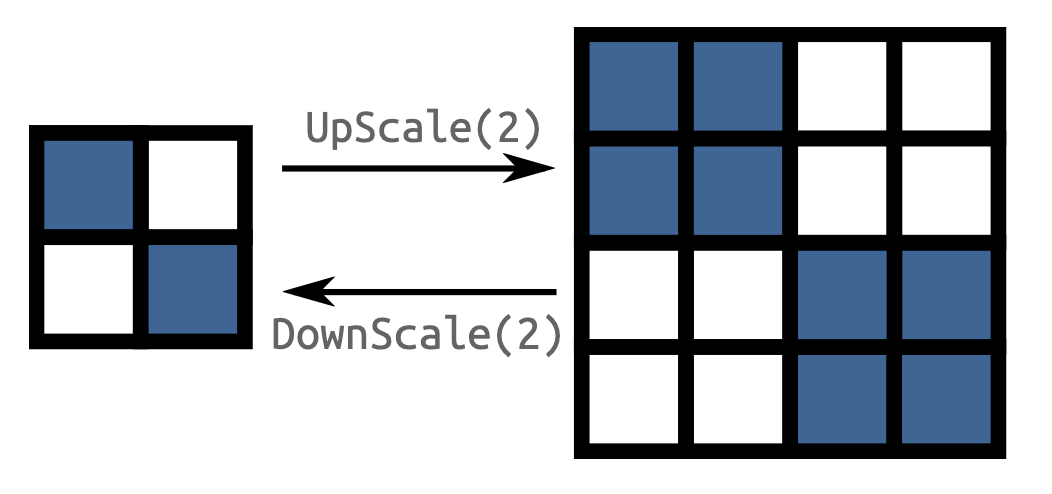
\includegraphics[width=0.5\linewidth]{scaling.png}
\end{center}

\end{document}